\documentclass[a4paper, 12pt]{article}

%%%%%%%%%%%%
% Packages %
%%%%%%%%%%%%

\usepackage[english]{babel}
\usepackage{packages/sleek}
\usepackage{packages/sleek-title}
\usepackage{hyperref}
\usepackage{placeins}
\usepackage{tikz}
\usepackage{booktabs,caption}
\usepackage{threeparttable}
\usepackage{listings}
\usepackage{xcolor}

%%%%%%%%%%%%%%%
% Definitions %
%%%%%%%%%%%%%%%

\definecolor{coderosewater}{RGB}{244, 219, 214}
\definecolor{codeflamingo}{RGB}{240, 198, 198}
\definecolor{codepink}{RGB}{245, 189, 230}
\definecolor{codemauve}{RGB}{136, 57, 239}
\definecolor{codered}{RGB}{237, 135, 150}
\definecolor{codemaroon}{RGB}{238, 153, 160}
\definecolor{codepeach}{RGB}{245, 169, 127}
\definecolor{codeyellow}{RGB}{238, 212, 159}
\definecolor{codegreen}{RGB}{166, 218, 149}
\definecolor{codeteal}{RGB}{139, 213, 202}
\definecolor{codesky}{RGB}{145, 215, 227}
\definecolor{codesapphire}{RGB}{125, 196, 228}
\definecolor{codeblue}{RGB}{30, 102, 245}
\definecolor{codelavender}{RGB}{183, 189, 248}
\definecolor{text}{RGB}{76, 79, 105}
\definecolor{subtext1}{RGB}{184, 192, 224}
\definecolor{subtext0}{RGB}{165, 173, 203}
\definecolor{overlay2}{RGB}{147, 154, 183}
\definecolor{overlay1}{RGB}{140, 143, 161}
\definecolor{overlay0}{RGB}{110, 115, 141}
\definecolor{surface2}{RGB}{91, 96, 120}
\definecolor{surface1}{RGB}{73, 77, 100}
\definecolor{surface0}{RGB}{54, 58, 79}
\definecolor{codebase}{RGB}{239, 241, 245}

\lstdefinestyle{CStyle}{
    backgroundcolor=\color{codebase},   
    commentstyle=\color{overlay1},
    keywordstyle=\color{codemauve},
    numberstyle=\tiny\color{codeblue},
    stringstyle=\color{codeflamingo},
    basicstyle=\footnotesize\color{text},
    breakatwhitespace=false,         
    breaklines=true,                 
    captionpos=b,                    
    keepspaces=true,                 
    numbers=left,                    
    numbersep=5pt,                  
    showspaces=false,                
    showstringspaces=false,
    showtabs=false,                  
    tabsize=2,
    language=C
}


%%%%%%%%%%%%%%
% Title-page %
%%%%%%%%%%%%%%

\logo{./resources/jpg/IMG_9668.jpg}
\institute{Brown University}
\faculty{Alex Khosrowshahi (Class of 2027)}
%\department{Department of Anything but Psychology}
\title{CS300: A Student's Guide}
\subtitle{Collected Notes and Reflections for my Favorite Class}
%\supervisor{Linus \textsc{Torvalds}}
\context{Yes, that is me in the photo}
\date{\today}

%%%%%%%%%%%%%%%%
% Resources %
%%%%%%%%%%%%%%%%

% Add helpful links here

%%%%%%%%%%%%
% Document %
%%%%%%%%%%%%

\begin{document}
\maketitle

\begin{center}


	\vfill
	\section*{The Purpose of this Document}

	This document is not meant to replace CS300's lecture notes, nor is it meant to replace lecture itself.
	If you want to do well, attend all lectures and ask questions. Go to hours. Go to section. Do your work. Your efforts will not go unrewarded.
	This document is also not restricted to in-order reading. Refer to whatever you need help with at a given time, set it down, and come back once you need help again.
	The lecture notes are probably better than I am.

	\vfill

	\clearpage

\end{center}

\section*{Preface}

\begin{flushleft}
	\makebox[\linewidth]{\rule{\paperwidth}{0.4pt}}
	\textbf{CS300 is not an easy class.}

	Quite the contrary---you will more than likely find yourself pulling long nights of head-scratching work for it if you share the lack of time management skills typical to
	computer science students. That said, it is one of the finest introductions to computer systems design, implementation, and, most importantly, principles that a student can experience.
	CS300 is hard because computer systems is a challenging subject---one that many of the greatest minds in computer science have and continue to grapple with daily.

	I say this because I do not want you to be discouraged by the hardships you may face. My advice is that when you become frustrated, step away for a moment and think about
	why you are here---what this whole systems thing is about. To build a computer has never been an easy task, and yet we do it despite adversity.

	To borrow the words of the brilliant Clifford Stoll, "Math ain’t about numbers. If you think math is about numbers, you probably think that Shakespeare is all about words.
		[...] Math ain’t about numbers. Math is about logic, it’s about beauty, it’s about connections, it’s about how you get from one place to another." Though we may not wear our
	mathematician hats in this course, I encourage you to adopt a similar sense of intellectual whimsy navigating this subject. As you learn about the internal mechanisms that
	drive electronic devices you use---of caching buffers, page tables, and other implementations we will discuss, you will find that your computer is full of stories; these stories
	are of mammoth challenges and the great minds that overcame them. Take moments to appreciate these recondite narratives---there is much beauty in the everyday machines we use.

\end{flushleft}

\romantableofcontents

\section{Memory, Data Types, and Pointers, Oh My!}
\begin{flushleft}
	By the time you take CS300, you hopefully have some fluency with a computer. You probably can make some decent projects with some boilerplate code or from scratch (good on you),
	you probably know the names of basic data types and what a constructor does, and you probably have some experience using an IDE, whether VSCode, IntelliJ, vim, emacs, or some other development tool.

	These are all imperative skills to have and ones that you'll need going forward, but up until now, you have been unknowingly working through many levels of abstraction. When you
	initialize a String, you don't think much about the space that string takes up. When you delete a node from a LinkedList in Java, inbuilt garbage collection handles the nastiness
	of cleaning up your computer memory. In this course, you'll learn what's going on under the hood of your computer---firstly, with understanding how data is stored.

\end{flushleft}
\subsection{Bits and Bytes}
\label{subsec:bitsbytes}
\begin{flushleft}

	Your computer's memory is formed out of \textbf{bytes}. Bytes are segments of 8 bits. A bit is an atomic unit of data with two modes, on or off, 1 or 0. Each byte, comprised of 8 bits,
	can hold \(2^8 =  256\) values. This means that within every byte we can store \textbf{any number between 0 and 255.}

	Every byte of memory in your computer has an address, one for each byte of memory. Professor Schwarzkopf and Professor DeMarinis like to describe these like post-office boxes, each storing some
	mail (value) and each having an address.
	\newline
\end{flushleft}

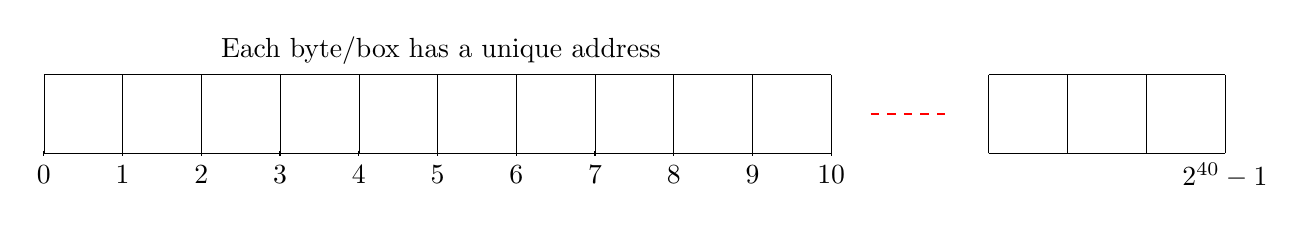
\begin{tikzpicture}
	\draw[step=1cm,black,very thin] (0,0) grid (10,1);
	\foreach \x in {0,1,2,3,4,5,6,7,8,9,10}
	\draw (\x cm,1pt) -- (\x cm,-1pt) node[anchor=north] {$\x$};
	\node[anchor=south] at (current bounding box.north) {Each byte/box has a unique address};
	\draw[red, thick, dashed] (10.5, 0.5) -- (11.5, 0.5);
	\draw[step=1cm,black,very thin] (12,0) grid (15,1);
	\node[anchor=north] at (15, 0) {$2^{40} - 1$};
\end{tikzpicture}

\subsection{Types and Sizes}

\begin{flushleft}
	Looking at a computer's memory this way, we stumble upon a surprisingly profound realization: all computer memory is the same.
	The data "types" we use are simply expressions of how much memory we're operating with and what information we store in said memory.
	For example, we can fit all commonly used English characters* within one byte of memory, with 256 unique identifiers, so a char is only one byte.
	An integer uses 4 bytes, giving us a range (from $2^0 \rightarrow 2^{32}$ if unsigned). One of the greatest strengths of C
	is the ability to work with memory on a deep level, so knowing your types and exactly how much memory they take up
	can be helpful.

	\begin{table}
		\centering
		\begin{threeparttable}
			\label{tab:datatypes}
			\caption{Data Types in C}
			\begin{tabular}{||c c c||}
				\hline
				Type             & Size         & Value Range                                                                               \\ [0.5ex]
				\hline\hline
				char (signed)    & 1 Byte       & -128 to 127                                                                               \\ [1ex]
				char (unsigned)  & 1 Byte       & 0 to 255                                                                                  \\ [1ex]
				short (signed)   & 2 Bytes      & -32,768 to 32,767                                                                         \\ [1ex]
				short (unsigned) & 2 Bytes      & 0 to 65,535                                                                               \\ [1ex]
				int (signed)     & 4 Bytes      & -2,147,483,648 to 2,147,483,647                                                           \\ [1ex]
				int (unsigned)   & 4 Bytes      & 0 to 4,294,967,295                                                                        \\ [1ex]
				long (signed)    & 4 or 8 Bytes & \href{https://www.tutorialspoint.com/c_standard_library/limits_h.htm}{See here, very big} \\ [1ex]
				long (unsigned)  & 4 or 8 Bytes & 0 to $2^{64}$ if 8 bytes                                                                  \\ [1ex]
				pointer          & 8 Bytes      & 0 to $2^{64}$ (all addressable memory)                                                    \\ [1ex]
				\hline
			\end{tabular}
			\begin{tablenotes}
				\small
				\item Note: long sizes differ by architecture, in CS300 assume 8 byte longs in C. Signed/unsigned means inclusive of negatives or noninclusive. See section 4 for more on signedness.
			\end{tablenotes}
		\end{threeparttable}
	\end{table}
	\FloatBarrier

	You may see something a little unfamiliar here---that being a "pointer," along with the conspicuous absence of Strings. Don't worry, we'll get there soon.
	What you need to understand right now is that all memory is the same, memory types are determined by the size of memory blocks
	allocated to store some data, and each memory type has a certain range of values it can store.

\end{flushleft}

\subsection{What's a Pointer?}

\begin{flushleft}
	We can store more than just data types like ints, longs, floats, and shorts in our 8-byte memory boxes---we can  also store the addresses
	of other memory! To do this, we use pointers.
	\newline
	\newline
	\textbf{Pointers are 8-byte segments of memory that hold other memory addresses within them.} The name "pointer" comes from thinking of these
	memory boxes as containing arrows pointing to other memory boxes. \textit{Pointers must also be stored in memory, and take up 8 bytes per pointer}.
\end{flushleft}

\subsubsection{Thank your lucky stars (dereferencing)}

\begin{flushleft}

	In C, we use two operators with pointers. The ampersand, \&, which gives the address of an item of data and the asterisk, *, which can mean two things:
	\begin{enumerate}
		\item An asterisk after a data type refers to a pointer, the type of data it points to depending on the type before the asterisk (e.g. an int* points to an integer)
		\item An asterisk before a pointer 'dereferences' that pointer, giving us access to the information stored in the address it points to.
	\end{enumerate}

	Pointers can be useful in C, which is a pass-by-value language, to pass memory between functions without duplication (among many other uses).
\end{flushleft}

\subsubsection{Array Pointer Duality}

\begin{flushleft}
	Arrays are not what they seem\dots
	\newline\newline
	In reality, \textbf{arrays in C are silently replaced with a pointer to the first element of an array in memory}---this means that in an array of 10 items, say 10 chars, the name itself
	for the array is actually a pointer to the start of a 10-byte region of memory with ten 1-byte blocks sequentially allocated in memory.
	\newline\newline
	\textbf{Strings are a lie too!}---a String is actually just a char array of however many characters are in the string + 1. Why the extra one?
	We reserve this spot for the null bit, indicating the location where a string terminates.

	\begin{lstlisting}[style=CStyle]
    import<stdio.h>

    int main(void) {
        // myArr actually decomposes to a pointer to the beginning of a
        // 40-byte segment of memory.
        int myArr[10] = {1, 2, 3, 4, 5, 6, 7, 8, 9, 10};
        // This means that if we define a pointer p
        int* p;
        // And assign it to myArr
        p = myArr;
        // C goes behind the scenes and decomposes the name myArr
        // to something like
        p = &myArr[0];
    }
    \end{lstlisting}

	\FloatBarrier
	The other tool you likely have or will use in class provided by array-pointer duality is pointer arithmetic.\footnote{Alex actually used pointer arithmetic in his entire initial implementation of DMalloc, only realizing he could use C
		arrow notation a few days before the due date. Please don't do this!}
	In case you need a reminder of how to use pointer arithmetic, we use the equation $$p[i] = *(p + (i \cdot \text{sizeof}(p)))$$ To navigate memory, where i is the number of steps we want
	to move forward in memory (or the index), p is the pointer we're performing pointer arithmetic on, and sizeof($p$) is the size of the data type we're performing pointer arithmetic on. C will, by default,
	include the size of your unit, so unless you're incrementing by a different data type's size (which you may need), you can only include $*(p + i)$.

	\begin{table}[]
		\centering
		\caption{Pointers: What to Remember}
		\begin{tabular}{|l|l|}
			\hline
			Operator + Name Combination                                  & Meaning                                                                   \\ \hline
			\&\textless{}name\textgreater{}                              & The address of the item with a given name                                 \\ \hline
			\textless{}type\textgreater{}* \textless{}name\textgreater{} & A \textless{}type\textgreater pointer named \textless{}name\textgreater{} \\ \hline
			*\textless{}name\textgreater{}                               & Dereferencing a pointer                                                   \\ \hline
		\end{tabular}
	\end{table}
\end{flushleft}

% Finished on 6/4/2024 - About 2 days elapsed

\newpage

% Started 6/21/2024 - Making slow progress

\section{Placing things (Where does it all go?)}

\begin{flushleft}
	Computers have very purposeful rules not only for how memory is used (you'll notice that \textit{purpose} is a common theme in this guide), but where it is used.
	In the following section, we'll quickly cover the different sections of memory, their uses,
	and how segments of memory are aligned for efficient use.
\end{flushleft}

\subsection{Sections of Memory}

\begin{flushleft}
	Your computer memory is separated into sections, each with different use cases. Why is this? There are many reasons:
	\begin{enumerate}
		\item For organization and consistency - Your computer can know where to go to find certain variables, values, etc.
		\item For safety of memory - Isolating segments of memory makes sure processes that shouldn't have access to certain memory remain contained.
		\item For performance - Again, reduction of searching Scoped
		\item For internal fragmentation - Related to performance, see \href{https://www.geeksforgeeks.org/internal-fragmentation-in-os/}{here}
	\end{enumerate}
	The four segments of memory are the \textbf{Code (or Text), Data, Stack, and Heap}. The uses of these segments are as follows:
	\begin{enumerate}
		\item The \textbf{Code/Text} is the section of memory that includes \textit{executable instructions} and \textit{constant global variables}.
		\item The \textbf{Data} is the section of memory that includes \textit{global variables}.
		\item The \textbf{Stack} is the section of memory that includes \textit{local variables}.
		\item The \textbf{Heap} is the section of memory that includes{\textit{dynamically allocated memory}}.
	\end{enumerate}
\end{flushleft}

\subsection{Alignment and Why We Do It}

\begin{flushleft}
	As we discussed in \hyperref[subsec:bitsbytes]{section 1}, different types of memory of different sizes are stored in "blocks" of bytes.
	Different types will have \hyperref[tab:datatypes]{blocks of different sizes}.
	\newline\newline
	This is all well and good, but actual operations on memory in your computer are often done in CPU cache. This is a small, hyper-fast segment of memory used
	for frequent, small operations. In x86 systems, the CPU cache is generally 64 bits, but different systems may vary. What we call \textit{alignment} is the manner
	by which your compiler aligns data in memory such that the CPU cache is optimally used.
\end{flushleft}

\newpage

\subsubsection{Alignment Rules for Common Types}
% TODO: Maybe do this, maybe leave it to the notes. Probably leave it to the notes.
\begin{flushleft}
	In order to keep alignment efficient, the C compiler aligns data in memory dependent on the data's type.
	This is done automatically when compiler optimizations are turned on, but it's good to keep these rules in mind
	when programming in memory-unsafe languages.
	\newline\newline
	For common types, alignment is relatively simple---common types must be aligned on a multiple of their size.
	Think of the boxes of bytes we use to represent memory---we want 4-byte integers to fall on multiples of 4,
	8-byte longs to fall on multiples of 8, etc.\footnote{Keep in mind, these multiples will be in hexadecimal since memory is in hex.}

\end{flushleft}

\begin{table}
	\centering
	\begin{threeparttable}
		\label{tab:alignmentcom}
		\caption{Alignment of Common Types in C}
		\begin{tabular}{||c c c||}
			\hline
			Type    & Size         & Address restriction \\ [0.5ex]
			\hline
			hline
			char    & 1 Byte       & No restriction      \\ [1ex] 
			short   & 2 Bytes      & Multiple of 2       \\ [1ex]
			int     & 4 Bytes      & Multiple of 4       \\ [1ex]
			long    & 4 or 8 Bytes & Multiple of 4 or 8  \\ [1ex]
			float   & 4 Bytes      & Multiple of 4       \\ [1ex]
			double  & 8 Bytes      & Multiple of 8       \\ [1ex]
			pointer & 8 Bytes      & Multiple of 8       \\ [1ex]
			\hline
		\end{tabular}
		\begin{tablenotes}
			\small
			\item Note: long sizes differ by architecture, in CS300 assume 8 byte longs in C.
		\end{tablenotes}
	\end{threeparttable}
\end{table}
\FloatBarrier

\begin{flushleft}

\end{flushleft}

\subsubsection{Struct Alignment Rules}
\begin{enumerate}
	\item
\end{enumerate}
\newpage

\section{Remember Me (Topics in Memory)}
\label{sec:dynamicmem}
\subsection{How does C allocate dynamic memory?}
\subsubsection{Regarding malloc()}
\subsubsection{Regarding free()}
\subsection{Common Issues}
\subsubsection{Avoiding the SEGFAULT Menace}
\subsubsection{Leak Prevention + Good Memory Practice}

\newpage

\section{Defining Undefined Behavior}
\label{sec:undef}
\subsection{What is Undefined Behavior?}
\subsection{Common Areas for Undefined Behavior}
\subsection{Dealing with Undefined Behavior}

\newpage

\section{Avengers, Assembly!}
\label{sec:assemblystuff}
\subsection{How Compiling Works}
\subsection{Reading Assembly}
\subsubsection{Assembly Cheat Sheet}
% Make a new one or link old one?

\newpage

\section{Racks on Racks, Stacks on Stacks (How the stack works)}
\label{sec:stackstuff}
\subsection{What is the Stack}
\subsection{Stack Organization}
\subsubsection{Special Registers}
\subsection{Stack Smashing}
\subsubsection{Buffer Overflows}

\newpage

\section{Operating the System}
\label{sec:os}
\subsection{What is an Operating System?}
\subsection{Privilege Separation/Memory Protection}
\subsection{Virtual Memory/Address Translation}
\subsection{Process Creation}
\subsubsection{The fork() syscall}
\subsubsection{The exec() syscall}

\newpage

\section{Inter-Process Communication}
\label{sec:ipcom}
\subsection{Introduction to Multiprocessing}
\subsection{Methods of Inter-Process Communication}
\subsubsection{waitpid()}
\subsubsection{Let's talk Pipes}

\newpage

\section{Beyond the Pipe: Concurrency, Parallelism, and Threads}
\label{sec:concstuff}
\subsection{Principles of Concurrency and Parallelism}
\subsection{Introduction to Multithreading}
\subsection{Race Conditions and Mutexes}
\subsection{Synchronization and Atomics}
\subsubsection{Bounded Buffer}
\subsection{Scoped Locks}

\newpage

\section{Wrapping Things Up}
\label{sec:ending}
\subsection{Our History as Computer Scientists}
\subsection{Philosophical Reflections}
\subsection{Further Reading}

\newpage

\section{Acknowledgements}
\label{sec:acknow}
\thispagestyle{empty}

% I would like to make a few acknowledgements:
% \newline
% First, Professor Malte Schwarzkopf and Professor Nick DeMarinis, for fostering such an incredible learning environment.
% \newline\newline
% I would also like to acknowledge my lecture buddy and CS300 Discord server co-leader, Nadia Sherman
% \newline My Caching I/O all-nighter partner Soujanya Aryal
% \newline And all my other friends from Spring 2024's CS300 section. What a gift it is to be here. 

% \begin{tikzpicture}
%     \filldraw[fill=red!40!white, draw=black] (0, 0) -- (0, 10) -- (7, 10) -- (7, 0) -- (5, 0) -- (5, 3) -- (2, 3) -- (2, 0) -- cycle;
%     \filldraw[fill=blue!30!white, draw=black] (0, 8) -- (4, 8) -- (4, 6) -- (0,6) -- cycle;
%     \fill[fill=white] (2, 7) -- (3, 7) -- (3, 7.5) -- (2, 7.5) -- cycle;
%     \filldraw[fill=red!40!white, draw=black] (7, 4) -- (9, 4) -- (9, 8) -- (7, 8) -- cycle;

% \end{tikzpicture}

\clearpage

\appendix

\end{document}
